
\chapter{Speculative Decoding}
\label{sec:speculative_decoding}

The academic part of this thesis revolves around speculative decoding. This chapter provides details around speculative decoding and the current landscape of research. It serves as context for the next chapter, where our new model, CASD, is proposed. First we explain the context of speculative decoding, followed by how it works. Finally, we give an overview of the most recent advancements. 

\section{Context of speculative decoding}

\begin{figure}[h]
	\centering
	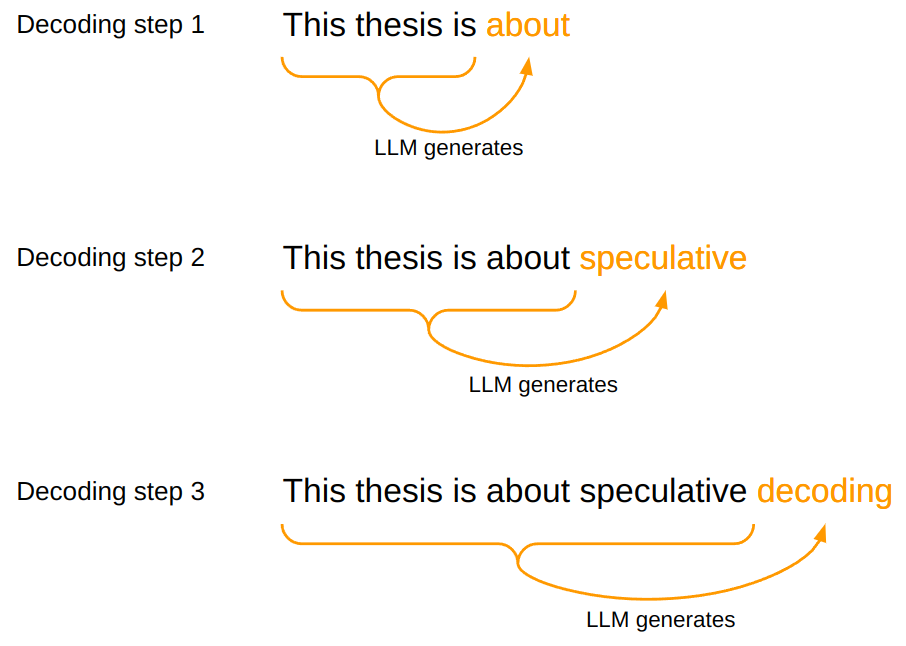
\includegraphics[width=0.7\linewidth]{fig/spec_dec_autoregressive.png}
	\caption{Autoregressive decoding by standard LLM.}
	\label{fig:spec_dec_autoregressive}
\end{figure}

To understand the need for speculative decoding, one must first understand the usual way of decoding with LLMs. Figure \ref{fig:spec_dec_autoregressive} shows the normal, autoregressive way of decoding. Autoregressive means that the LLM ``reads'' all previous tokens to generate the next token. So to construct an answer, the LLM takes the input and generates one new token. Then it takes the input and the new token and generates another new token. This is repeated until the LLM decides the answer is complete or the maximal output length is reached.

The inefficiency of this autoregressive decoding is that it does not use the full capacity of the GPU it is running on. While GPUs are very complex, we can still simplify their limitations to two constraints. On the one hand, a GPU has limited computing power, which means it can only do so many operations per second. On the other hand, GPUs can only load a limited amount of data per second. Surprisingly, the latter constraint is the real bottleneck for LLMs. This is because each time the LLM is called (each generation step from before), the LLM parameters need to be loaded from the VRAM to the GPU. This large amount of data seems to be slower to transfer than the actual time the GPU needs to compute the results. In other words, the GPU could calculate faster, but loading the model each time keeps it from doing so.

There are two types of solutions for this bottleneck. The first one is relevant to the larger players in the market. Suppose an LLM host receives many requests per second. In this case, the questions can be batched, as shown in Figure \ref{fig:spec_dec_batch}. This means that the server waits for a certain number of questions to arrive, before processing them all together, in parallel. The effect is that the model is only loaded once into the GPU, while generating the next token for each of the questions. So if there are for example 16 questions in a batch, the GPU is calculating 16 times as much, while loading the same model only once. Thus, the calculation intensity is increased and much of the spare calculation-capacity is filled in. In conclusion, this method increases the GPU efficiency, by exploiting the many requests coming in per second.

\begin{figure}[h]
	\centering
	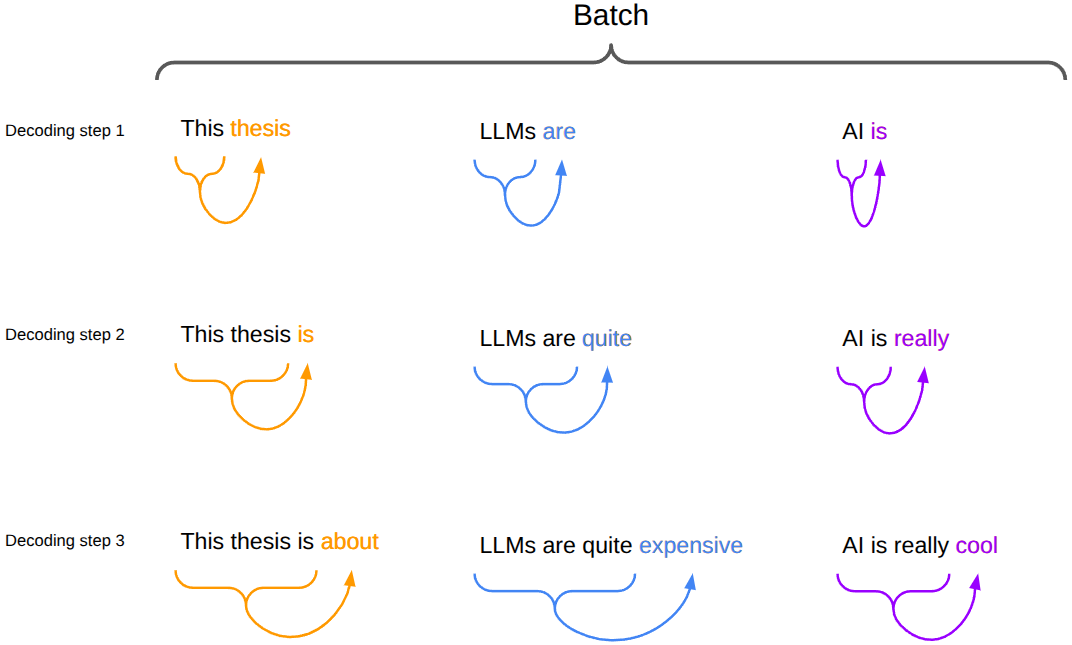
\includegraphics[width=1\linewidth]{fig/spec_dec_batch.png}
	\caption{Batch decoding on a small example. The different users' prompts are indicated with colors.}
	\label{fig:spec_dec_batch}
\end{figure}

The second solution to the GPU memory bottleneck is speculative decoding. Speculative decoding does not need the large load of requests per second to achieve parallelism. Instead, it tries to break the autoregressive nature of LLMs and to parallelize it. The following section describes how that works in detail.

\section{How does speculative decoding work?}

\begin{figure}[H]
	\centering
	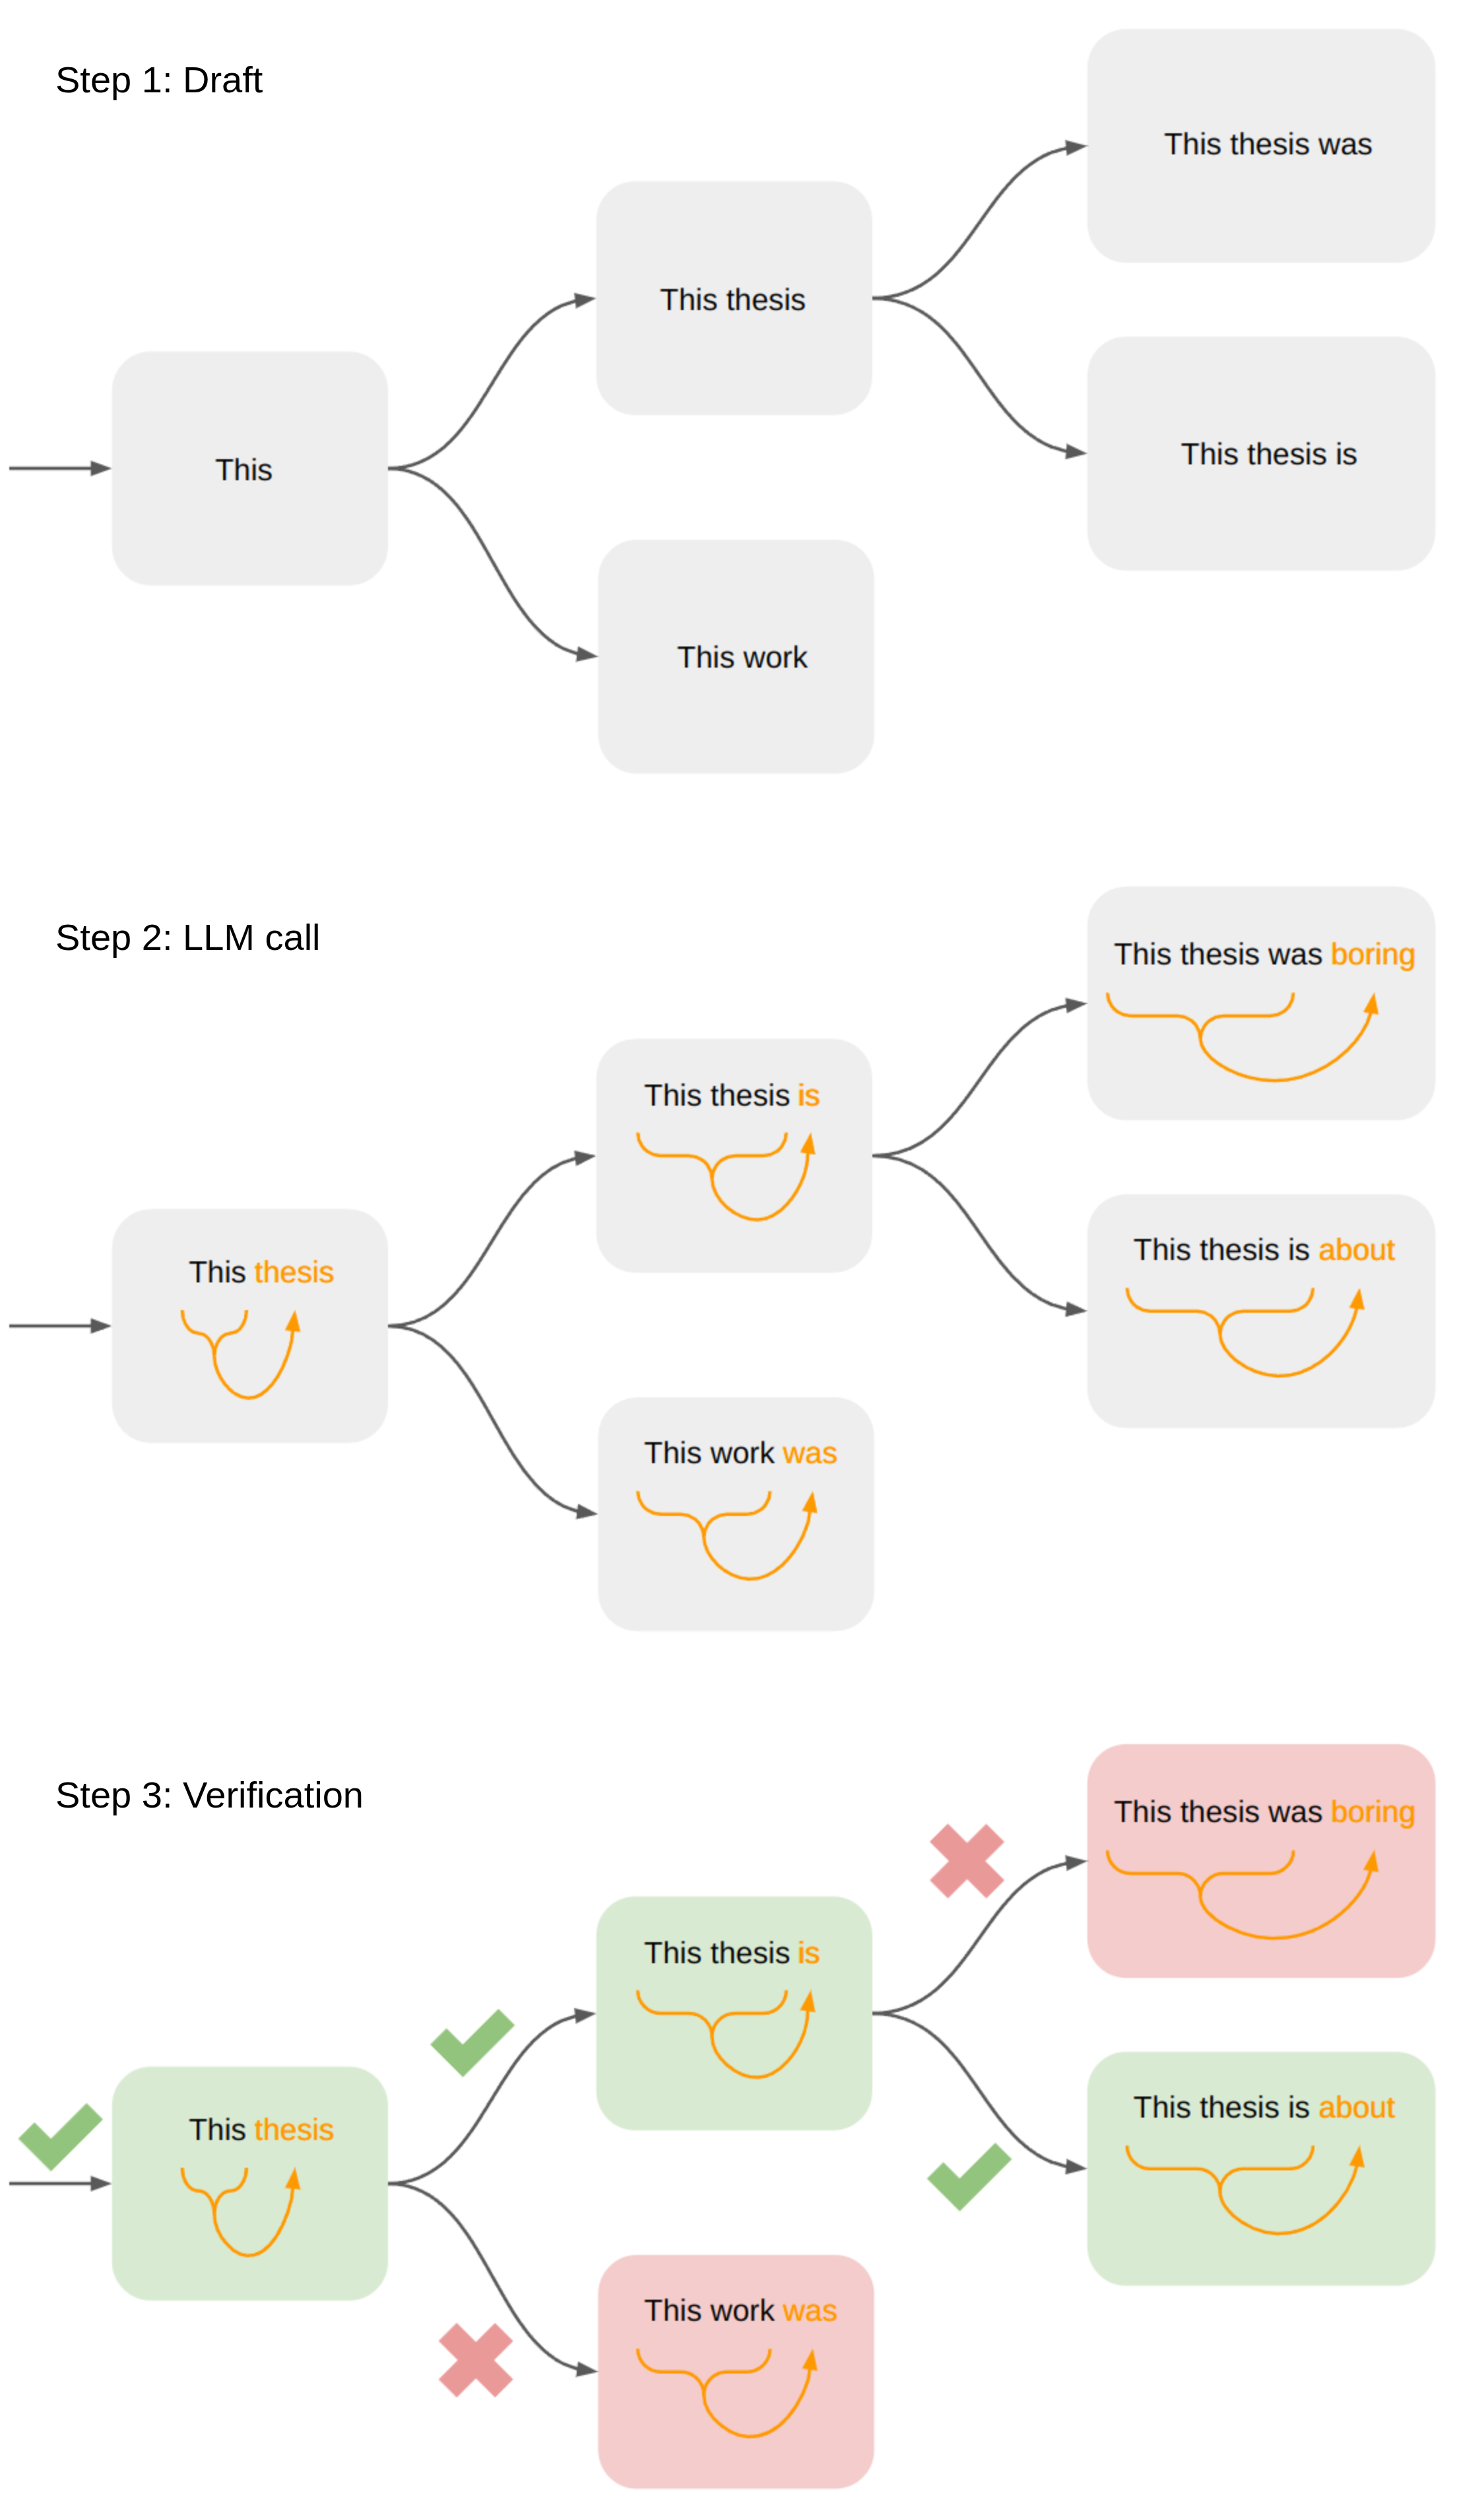
\includegraphics[width=0.75\linewidth]{fig/spec_dec_three_step_plan.png}
	\caption{Step-by-step explanation of speculative decoding: in step 1, the drafter makes a tree of possible outcomes. Each draft is the same as its parent plus one speculated token. In step 2, the LLM call determines which token would be generated next for each of the speculations. In step 3 each speculated token is verified. The longest correct speculation is accepted. Here that is ``This thesis is about''.}
	\label{fig:spec_dec_three_step_plan}
\end{figure}

Speculative decoding tries to form batches, but rather than looking at multiple users, it looks multiple decoding steps ahead. To do so, it follows a three-step plan. These steps are detailed below, with Figure \ref{fig:spec_dec_three_step_plan} as a guide.

The first step is to make a good guess (a.k.a. draft) what the LLM will generate, without calling the LLM itself. This step is the hardest step and by consequence the focus of most research in the domain. Many clever methods have been found already and we provide a short overview of them in Section \ref{sec:drafting_methods}. This thesis also focuses on the drafting.

In the second step, the guesses are verified in parallel. To do so, a tree is made of all predictions. In this tree, guesses with a common prefix are joined, such that the prefix has to be verified only once. Once the tree is made, each node of the tree needs to be run through the LLM to see what the correct token is at that step. When sending all tokens to the LLM, it must be sure that tokens from different guesses do not interfere with each other. This is made possible with tree attention. Tree attention puts a mask over the attention, such that tokens from other branches in the tree are "invisible" to the current branch. So to conclude, tree attention makes it possible to call the LLM only once, while verifying many guesses.

The third step is to accept the longest correct guess. A correct guess can have multiple interpretations. When the temperature is 0, it is easier to define. Temperature 0 means that the LLM will always, deterministically pick the most probable next word. In this case, correct means that the guess chose exactly the same tokens as the LLM. In the case of temperature different from 0, the answer is not deterministic anymore. So more calculations are involved to guarantee the output distribution is the same as the LLM would have chosen. As this sampling method is not the focus of this thesis, we do not explain it further and we limit the discussion to temperature equal to 0. 

One last remark must be made to fully understand the accept step. The real accepted length is always one larger than the longest accepted guess. How is that possible? Suppose we had no correct guesses, then we still called the LLM on the original output. Similarly, if we had n correct tokens, we also called the LLM on the n-th token and know what the n+1th token should be. This last part ensures one extra token is accepted each iteration.

\section{Drafting methods}
\label{sec:drafting_methods}
To understand the innovation of CASD, we must first look at the existing drafters and what their weaknesses are. The existing drafters can be divided into two categories: the statistical speculators and the neural speculators. Statistical techniques are more hand-crafted methods, while neural methods train a neural network to do the drafting. In this thesis, we will introduce a third category: the hybrids that combine statistical and neural methods. Below, we list some examples of recent work in the two standard categories.

Starting off with the statistical techniques: REST \cite{he2023rest} makes drafts by scanning existing text to find probable snippets. Practically, they use a large dataset of existing documents to find continuations of what is currently being generated. This is visualized in Figure \ref{fig:spec_dec_rest}. We also mention Inference with Reference \cite{yang2023inference}, not for its performance, but because it has similarities with the method we propose. Inference with Reference works similarly to REST, but instead of looking in a large dataset, it looks back at the prompt and the generated tokens to see if it is copying from its own context. Statistical models are typically very fast, but they do not generate the most accepted tokens on average. They are outperformed by the neural models, which are very good at predicting a few tokens very consistently. 

\begin{figure}[h]
	\centering
	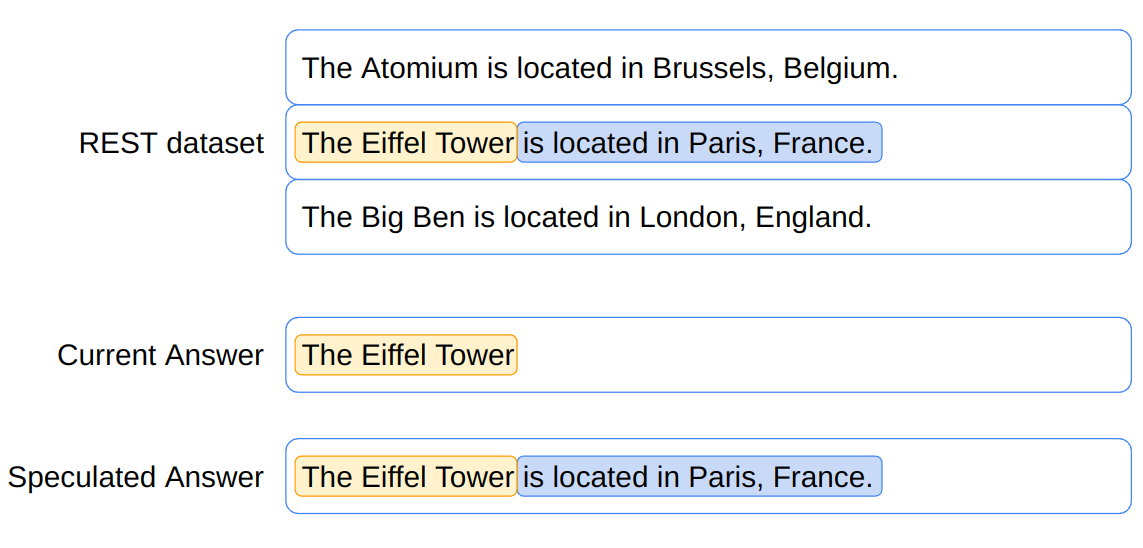
\includegraphics[width=0.7\linewidth]{fig/spec_dec_rest.png}
	\caption{Example of REST \cite{he2023rest} drafting. In the large dataset, REST found a match in the documents and it speculates the words that follow it in the document.}
	\label{fig:spec_dec_rest}
\end{figure}

The second category of drafters, the neural speculators, can be further subdivided based on their key ideas. The key idea of the earlier methods was to use a smaller LLM to speculate what the larger LLM would generate \cite{leviathan2023fast}. However, they do not exploit the features that are generated by the LLM ``for free''. These features contain valuable information, the thoughts of the LLM in a sense. So the key idea of most new models is to use the features generated by the LLM too, as an extra source of input. For example, the current state-of-the-art, EAGLE-2 \cite{li2024eagle}, tries to generate the next features autoregressively instead of generating the tokens directly. This is visualized in Figure \ref{fig:EAGLE_model}. The core weakness of neural speculators is that they are defined by their training set. If they are trained on English, they will probably work well only on English (as we show later). Thus, anything out-of-distribution can be a weak spot.

\begin{figure}[h]
	\centering
	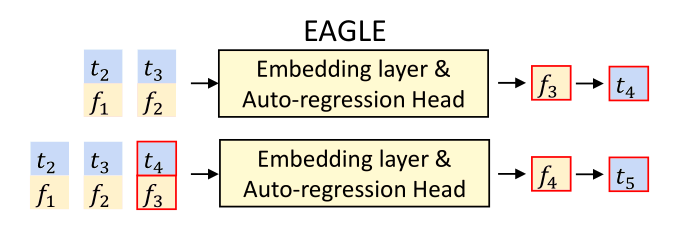
\includegraphics[width=0.7\linewidth]{fig/EAGLE_model.png}
	\caption{EAGLE-2 uses the LLM's \textcolor{orange-ish}{features} and previous \textcolor{blue-ish}{tokens} to predict the next step. It is used autoregressively, to draft multiple tokens ahead. Figure from EAGLE-2 \cite{li2024eagle}.}
	\label{fig:EAGLE_model}
  \end{figure}
